\chapter{Background} \label{Chapter:Background}

\section{Game Theory}

\subsection{Nash Equilibrium}
The concept of a Nash Equilibrium plays a central role in game theory. The definition in simple setting of a finite player is described as follow with mathematical form. Form indexes $K$ agents as $k=i, \dots, K$. There are total $N_k$ pure strategies. From $N_k$ agent k choose a strategy called $s_k$. $S_k$ denotes the set of strategies, and $s_k$ as the member of the set. A strategy profile, named $s = (s_1, ..., s_K)$, is a vector of strategies for the individual players. Hence, all strategy profiles can be written as $S$ for $\Pi_{k=1}^{K} S_{k}$. We write $s \mid s_{k}^{\prime}$ for the strategy $\left(s_{1}, \ldots, s_{k-1}, s_{k+1}^{\prime}, \ldots, s_{K}\right)$ means a strategy of agent $k$ changed from $s_k$ to $s_{k}^{\prime}$, in which a strategy profile $s$ is $s = (s_1, ..., s_K)$ and a strategy of agent $k$ is $s_{k}^{\prime} \in S_{k}$. The excepted utility or payoff of each agent $k$ is formed as $u_k(s)$, when agents select strategy profile $s$\parencite{Kreps1989}.
\begin{proposition}[Nash Equilibrium]
For a strategy profile $s$, Nash Equilibrium can be described by a mathematical inequalities: For each agent $k$ and $s_{k}^{\prime} \in S_{k}$, $u_{k}(s) \geqslant u_{k}\left(s \mid s_{k}^{\prime}\right)$.
\end{proposition}
In terms of words description, the definition of Nash Equilibrium is that if other agents do not change its strategy, then no single agent can obtain higher utility. 
 
\subsection{Pareto Efficient}
Pareto Efficient is also named as \textbf{Pareto Optimal} which is a state at which resources in a system are optimized in a way that one dimension cannot improve without a second worsening. We can consider an economy scenario, there are N agents and K goods. For an allocation state, formed as $x=\{x_1, \dots, x_n\}$, where $x_i \in \dsR^{K}$. $x_i$ represents the resource set allocated to each agent $i$. The utility of each agent $i$ is formed as $u_i(x_i)$. Therefore, the Pareto optimal allocation is defined as follows.

\begin{proposition}[Pareto Efficient]
There is no other feasible allocation $\{x_{1}^{\prime},...,x_{n}^{\prime}\}$ where, for 
utility function $u_i$ for each agent $i$, $u_{i}(x_{i}^{\prime}) \geqslant u_{i}(x_{i})$ for all $i \in \{1,...,n\}$ with $u_{i}(x_{i}^{\prime})>u_{i}(x_{i})$ for some $i$ \parencite{Whinston1989}.
\end{proposition}

The relationship between Pareto Efficient and Nash Equilibrium has following two points:

\begin{itemize}
\item A certain Nash Equilibrium will implement a resource allocation, which may or may not be Pareto optimal.
\item A certain Pareto Optimal resource allocation may or may not be obtained by the execution of the Nash Equilibrium of a completely information static game.
\end{itemize}

\subsection{Markov Games} \label{background-game-theory-markov-game}
These Games based on the \textbf{Markov Decision Process}(\gls{mdp}) are called Markov Game. The term \gls{mdp} has been proposed by Bellman in 1954\parencite{Bellma1954}. It can be described as a system that can be controlled by a sequential decisions.

\paragraph{Finite \gls{mdp} model}
means \gls{mdp} with finite time horizon. The model mainly includes the state space, action space, random transition law and reward function of the system. Hence, a non-stationary \gls{mdp} with horizon $N \in \dsN$ consists of a set of data $(S, A, D_n, Q_n, r_n, g_N)$ with the follwing meaning \parencite{Bäuerle2010}:

\begin{itemize}
\item $S$ is the state space, the elements(states) are denoted by $s \in S$
\item $A$ is the action space, the elements(actions) are denoted by $a \in A$.
\item $D_{n} \subset S \times A$ denotes the set of admissible state-action pairs at time $n$.
\item $Q_n$ is a stochastic transition kernel from $D_n$ to $S$. $Q_n$ describes the transition law. The quantity $Q_n(s^{\prime} \mid s, a)$ gives the probability that next state at time $n+1$ is $s^{\prime}$ if the current state is $s$ and action is $a$.
\item $r_n: D \rightarrow \dsR$ is a mapping function. Hence, at the time $n$, the reward of the system can be denoted by $r_n(s, a)$, where the state is $s$ and action is executed as $a$.
\item $g_N: E \rightarrow \dsR$ is a measurable mapping. $g_N(s)$ gives the discounted terminal reward of the system at the time $N$ if the state is $s$. 
\end{itemize}

Next step the definition of strategy(policy) is neccessary to be introduced. A strategy is a mapping $\pi: S \rightarrow A$, where $\pi(s)$ means the action an agent will perform in state $s$. In the case of a given MDP, the agent should adopt the best strategy, which should maximize the accumulated expected reward when performing the specified action. Since \gls{rl} is based on the \gls{mdp} process, how to find the optimal strategy and calculate the accumulated expected reward are important questions in the research field of \gls{rl}. All the details will be further introduced in the section value functions \ref{background:value-function}.

\paragraph{Multi-Agent Markov Decision Processes(\gls{mdps})} Based on communication ability of agent, multi-agent extension of \gls{mdps} can be called partially or complete observable markov games. There are $N$ players indexed by $n=1,2, \dots ,N$. A markov game for $N$ agents is defined by a set of states $S$ describing the possible configuration of all agents. $A_1, \dots, A_N$ and $O_1, \dots, O_N$ are the set of actions and observations of individuale agents, respectively. For each agent, a stochastic strategy $\boldsymbol{\pi}_{\theta_{i}}$ will be used to choose action, the mapping is $\boldsymbol{\pi}_{\theta_{i}}: \mathcal{O}_{i} \times \mathcal{A}_{i} \mapsto[0,1]$. For the multi-agent \gls{mdps}, the transition function is defined as following mapping functions $\mathcal{T}: \mathcal{S} \times \mathcal{A}_{1} \times \ldots \times \mathcal{A}_{N} \mapsto \mathcal{S}$, which produces the next state. The term $r_i(s, a)$ means the reward of agent $i$ if the state is $s$ and action $a$ is taken. The mapping of reward function is described as $r_i: S \times A_i \mapsto \dsR$. Each agent $i$ receives the private observation correlated with the state $o_i: S \mapsto O_i$\parencite{maddpg2017}. There are many cases for multi-agent \gls{mdps}. Following three items are the typical cases that are introduced by \texttt{Boutilier} in the paper\parencite{Boutilier1996PlanningLA}.
\begin{itemize}
\item Complete communication
\item Communication of actions, but not states 
\item No communication of actions or states
\end{itemize}

\section{Autonomous Negotiaion} \label{autonomous-negotiation}
Negotiation is an important process in coordinating behavior and represents a principal topic in the field of multi-agent system research. Extensive research has been conducted in the field of autonomous negotiation agent.

Automated agents can be used side-by-side with a human negotiator embarking on an important negotiation task. They can alleviate some of the effort required of people during negotiations and also assist people who are less qualified in the negotiation process. There may even be situations in which automated negotiators can replace the human negotiators. Thus, success in developing an automated agent with negotiation capabilities has great advantages and implications\parencite{Baarslag2012}.

Through the negotiation agents, many problems that arise in real or simulated domain can be solved. In industrial domains and in commerical domains, the supply chain management(\gls{scm}) system functionality is implemented through agent-based negotiation environment, in which contracts can be singed through negotiation between agents. Many papers describe ongoing effort in developing a Multi-agent System(\gls{mas}) for supply chain management, such as work in paper \parencite{Lee2004, Lin2014}.

\subsection{Utility Function}
\textbf{Utility Function} is an important concept in economics. It measures preferences for a set of goods and services. Utility Function can measure either single offer or set of offers.

Utility represents the satisfaction that consumers obtain when choosing and consuming products or services and is measured in units called utils, but calculating the benefit or satisfaction that consumers receive from is abstract and difficult to pinpoint\parencite{ANDRIY2019}. One typical utility function is briefly listed and introduced below:

\begin{itemize}
\item \textbf{linear utility function:} $u\left(x_{1}, x_{2}, \ldots, x_{m}\right)=w_{1} x_{1}+w_{2} x_{2}+\ldots w_{m} x_{m}$ or described as a vector $u(\vec{x})=\vec{w} \cdot \vec{x}$, where $m$ is the number of differen goods in the economy. The element $x$ represents the amount of good $i$. The element $w_i$ represents the relative value that the consumer assigns to good $i$.
\end{itemize}

It is a important point for designing a new agent in autonomous negotiation environment. For heuristic agents utility function is a keypoint to measure preferences. For reinforcement learning agents utility function conducts the behavior of learnable agents, and it can be used as a part of reward function, which significantly affects the design and evaluation of RL-agent.

\subsection{Basic Notation in Negotiation Mechanism} \label{background:autonmous-negotiation:basic-notation}
Before introducing a specific negotiation mechanism, it is necessary to understand some basic symbols defined in the paper \parencite{Aydoğan2017}.

\begin{definition}[Round and Phase]
Round and Phase within rounds are used to structure the negotiation process.
\end{definition}

\begin{definition}[Turn taking]
Protocols assign turns to the negotiating agents. Turns are taken according to a turn-taking sequence.
\end{definition}

\subsection{Rubinstein Bargaining Mechanism}
Rubinstein bargaining mechanism is widely cited for multi-round bilateral negotiation.
Two agents in the mechanism which has an infinite time horizon and have to reach an agreement. In a turn, one agent propose an offer, the other need to decide either to accept it, or to reject it and continue the bargaining\parencite{Rubinstein1982}. The offer is about how to divide the pie of size 1. After the two agents have played indefinitely, they may get the corresponding nash equilibrium solution.

\subsection{Stacked Alternating Offers Mechanism(\gls{saom})} \label{background:saom}
In the alternating offers protocol, one of the agent start to proposal an offer. The other can either accept or reject the given offer. If an agreement is reached, the negotiation is successful and ended. When rejecting the offer the other agent can either end the negotiation or give a count offer.

\gls{saom} is also named as stacked alternating offers protocol. Agents can only take their action when it is their turn. \gls{saom} allows negotiating agents to evaluate only the most recent offer in their turn and accordingly they can take the following actions:
\begin{itemize}
\item Make a count offer (thus rerejecting and overriding the previous offer)
\item Accept the offer
\item Walk away (e.g. ending the negotiation without any agreement)
\end{itemize}
This negotiation process is repeated until a termination condition is met. The termination condition is met, if an agreement is reached or the deadline is reached. When an agreement is reached, all agents need to accept the offer. If at the deadline no agreement is reached, this negotiation is failed. 

\section{Artificial Intelligence}
Artificial intelligence is a broad branch of computer science that is focused on a machine’s capability to produce rational behavior from external inputs. The goal of AI is to create systems that can perform tasks that would otherwise require human intelligence. It is generally believed that the field of artificial intelligence began at a conference held at Dartmouth College in July 1956, when the term "artificial intelligence" was first used\parencite{Brunette2009}.

There is a set of three related items that sometimes are erroneously used interchangeably, namely artificial intelligence, machine learning, and neural networks. According to Encyclopaedia Britannica, AI defines the ability of a digital computer or computer-controlled robot to perform tasks commonly associated with intelligent beings. On the other hand, according to Arthur Samuel, one of the pioneers of the field, machine learning is a “field of study that gives computers the ability to learn without being explicitly programmed”\parencite{Samuel1959, Bhavsar2017}.

\subsection{Sub-areas}
Fig. \ref{fig:ai_taxonomy} shows the relationship of artificial intelligence, machine learning and deep learning. AI is a program that can sense, reason, act and adapt. Machine learning is a set of methods, whose performance improve as they are exposed to more data over time.	Deep learning is a subset of machine learning, in which multi-layered neural networks learn from vast amount of data.

\begin{figure}[htbp]
\centering
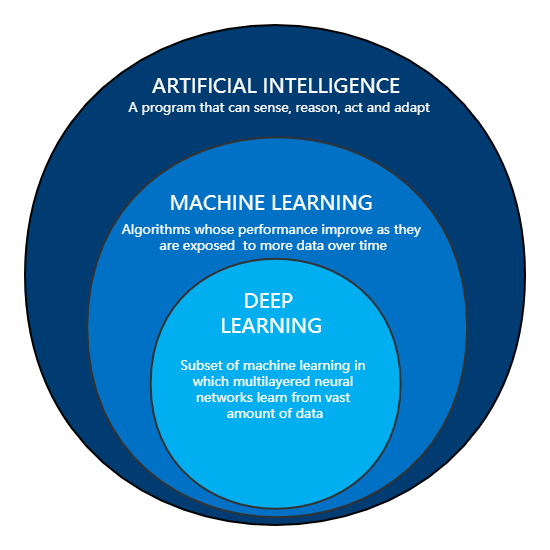
\includegraphics[width=0.4\textwidth]{./images/ai_taxonomy.png}
\caption{Sub-areas of artificial intelligence Source: Own illustration based
on\parencite{Suman2020}}
\label{fig:ai_taxonomy}
\end{figure}

\subsubsection{Artificial Intelligence}
Artificial intelligence (also called machine intelligence) can be understood through a type of intelligence, which is different from the natural intelligence displayed by humans and animals, which can be demonstrated by machines. It looks at methods for designing smart devices and systems that can creatively solve problems that are usually regarded as human privileges. Hence, AI means that the machine imitates human behavior in some way. 
\subsubsection{Machine Learning} 
Machine learning is an AI subset and consists of techniques that enable computers to recognize data and supply AI applications. Different algorithms (e.g., neural networks) contribute to problem resolution in ML.

\subsubsection{Deep Learning}
Deep learning, often called deep neural learning or deep neural network, is a subset of machine learning that uses neural networks to evaluate various factors with a similar framework to a human neural system. It has networks that can learn from unstructured or unlabeled data without supervision.

\subsection{Methods}
\paragraph{Supervised Learning}
Training data contains optimal outcomes (also known as inductive learning). Learning is tracked in this method. Some famous examples of supervised machine learning algorithms are Linear regression for regression problems. 
\paragraph{Unsupervised Learning} 
There are not the desired outputs in the training results. Clustering is an example. It is impossible to know what is and what is not good learning.
\paragraph{Semi-supervised Learning}
A few desired outputs are included in the training data.
\paragraph{Reinforcement Learning}
Rewards are given after a sequence of actions. In a given case, it is a matter of taking appropriate steps to maximize compensation. It is the most ambitious method of learning in AI.

\subsection{Application Field}
AI researchers have paid a great deal of attention to automated negotiation over the past decade and a number of prominent models have been proposed in the literature. Autonomous agent is an important concept of AI. AI is a big concept with a wide range of applications. It provides support for many scenarios, such as eCommerce, Logistics and Supply Chain and as research tools for computer science. In this section, some applications of autonomous negotiation based on AI will be introduced.

\subsubsection{eCommerce}
\paragraph{Rank in E-Commerce Search Engine} In E-commerce platforms such as Amazon and TaoBao, ranking items in a search session is a typical multi-step decision-making problem. AI can learn the relation between different ranking steps, in the paper
\parencite{Hu2018} authors use reinforcement learning (RL) to learn an optimal ranking policy, which maximizes the expected accumulative rewards in a search session. The more reasonable the ranking of commodities, the more frequent commodity transactions, and the greater the corresponding income.

\paragraph{Business-to-Business Negotiation} Negotiation is an important challenge for B2B eCommerce. For B2B e-commerce, AI is making great strides and is being used in a variety of ways to improve and enhance business\parencite{Hans01}. AI-based algorithms and tools can help companies in various ways, from personalizing the shopping experience to improving supply chain management.

\subsubsection{Logistics and Supply Chain}
\paragraph{Contextual Intelligence} AI provides contextual intelligence for the supply chain, and they can use contextual intelligence to reduce operating costs and manage inventory. Contextual information can help them return to customers quickly.   
\paragraph{Enhancing Productivity and Profits} AI can analyze the performance of the supply chain and propose new factors that affect the same field. It can combine the capabilities of different technologies such as reinforcement learning, unsupervised learning and supervised learning to discover factors and problems that affect the performance of the supply chain and can make better contracts between different suppliers and consumers\parencite{Pndey2019}. It can analyze the data related to the supplier like audits, in-full delivery performance, credit scoring, evaluations and based on that deliver information which can be used to make future decisions. This kind of step helps the company make better decisions as a supplier and work towards improving customer service. Autonomous negotiation by autonomous agent is an important technology that can be used in this field.

\section{Artificial Neural Network (\gls{ann})}
Artificial neural network is a technology based on the study of the brain and nervous system\parencite{WALCZAK2003631}. \gls{ann}s are efficient data-driven modelling tools widely used for nonlinear systems dynamic modelling and identification, due to their universal approximation capabilities and flexible structure that allow to capture complex nonlinear behaviors \parencite{SHOKRY2018265}. 

\subsection{Artificial Neuron}


\begin{figure}[htbp]
\centering
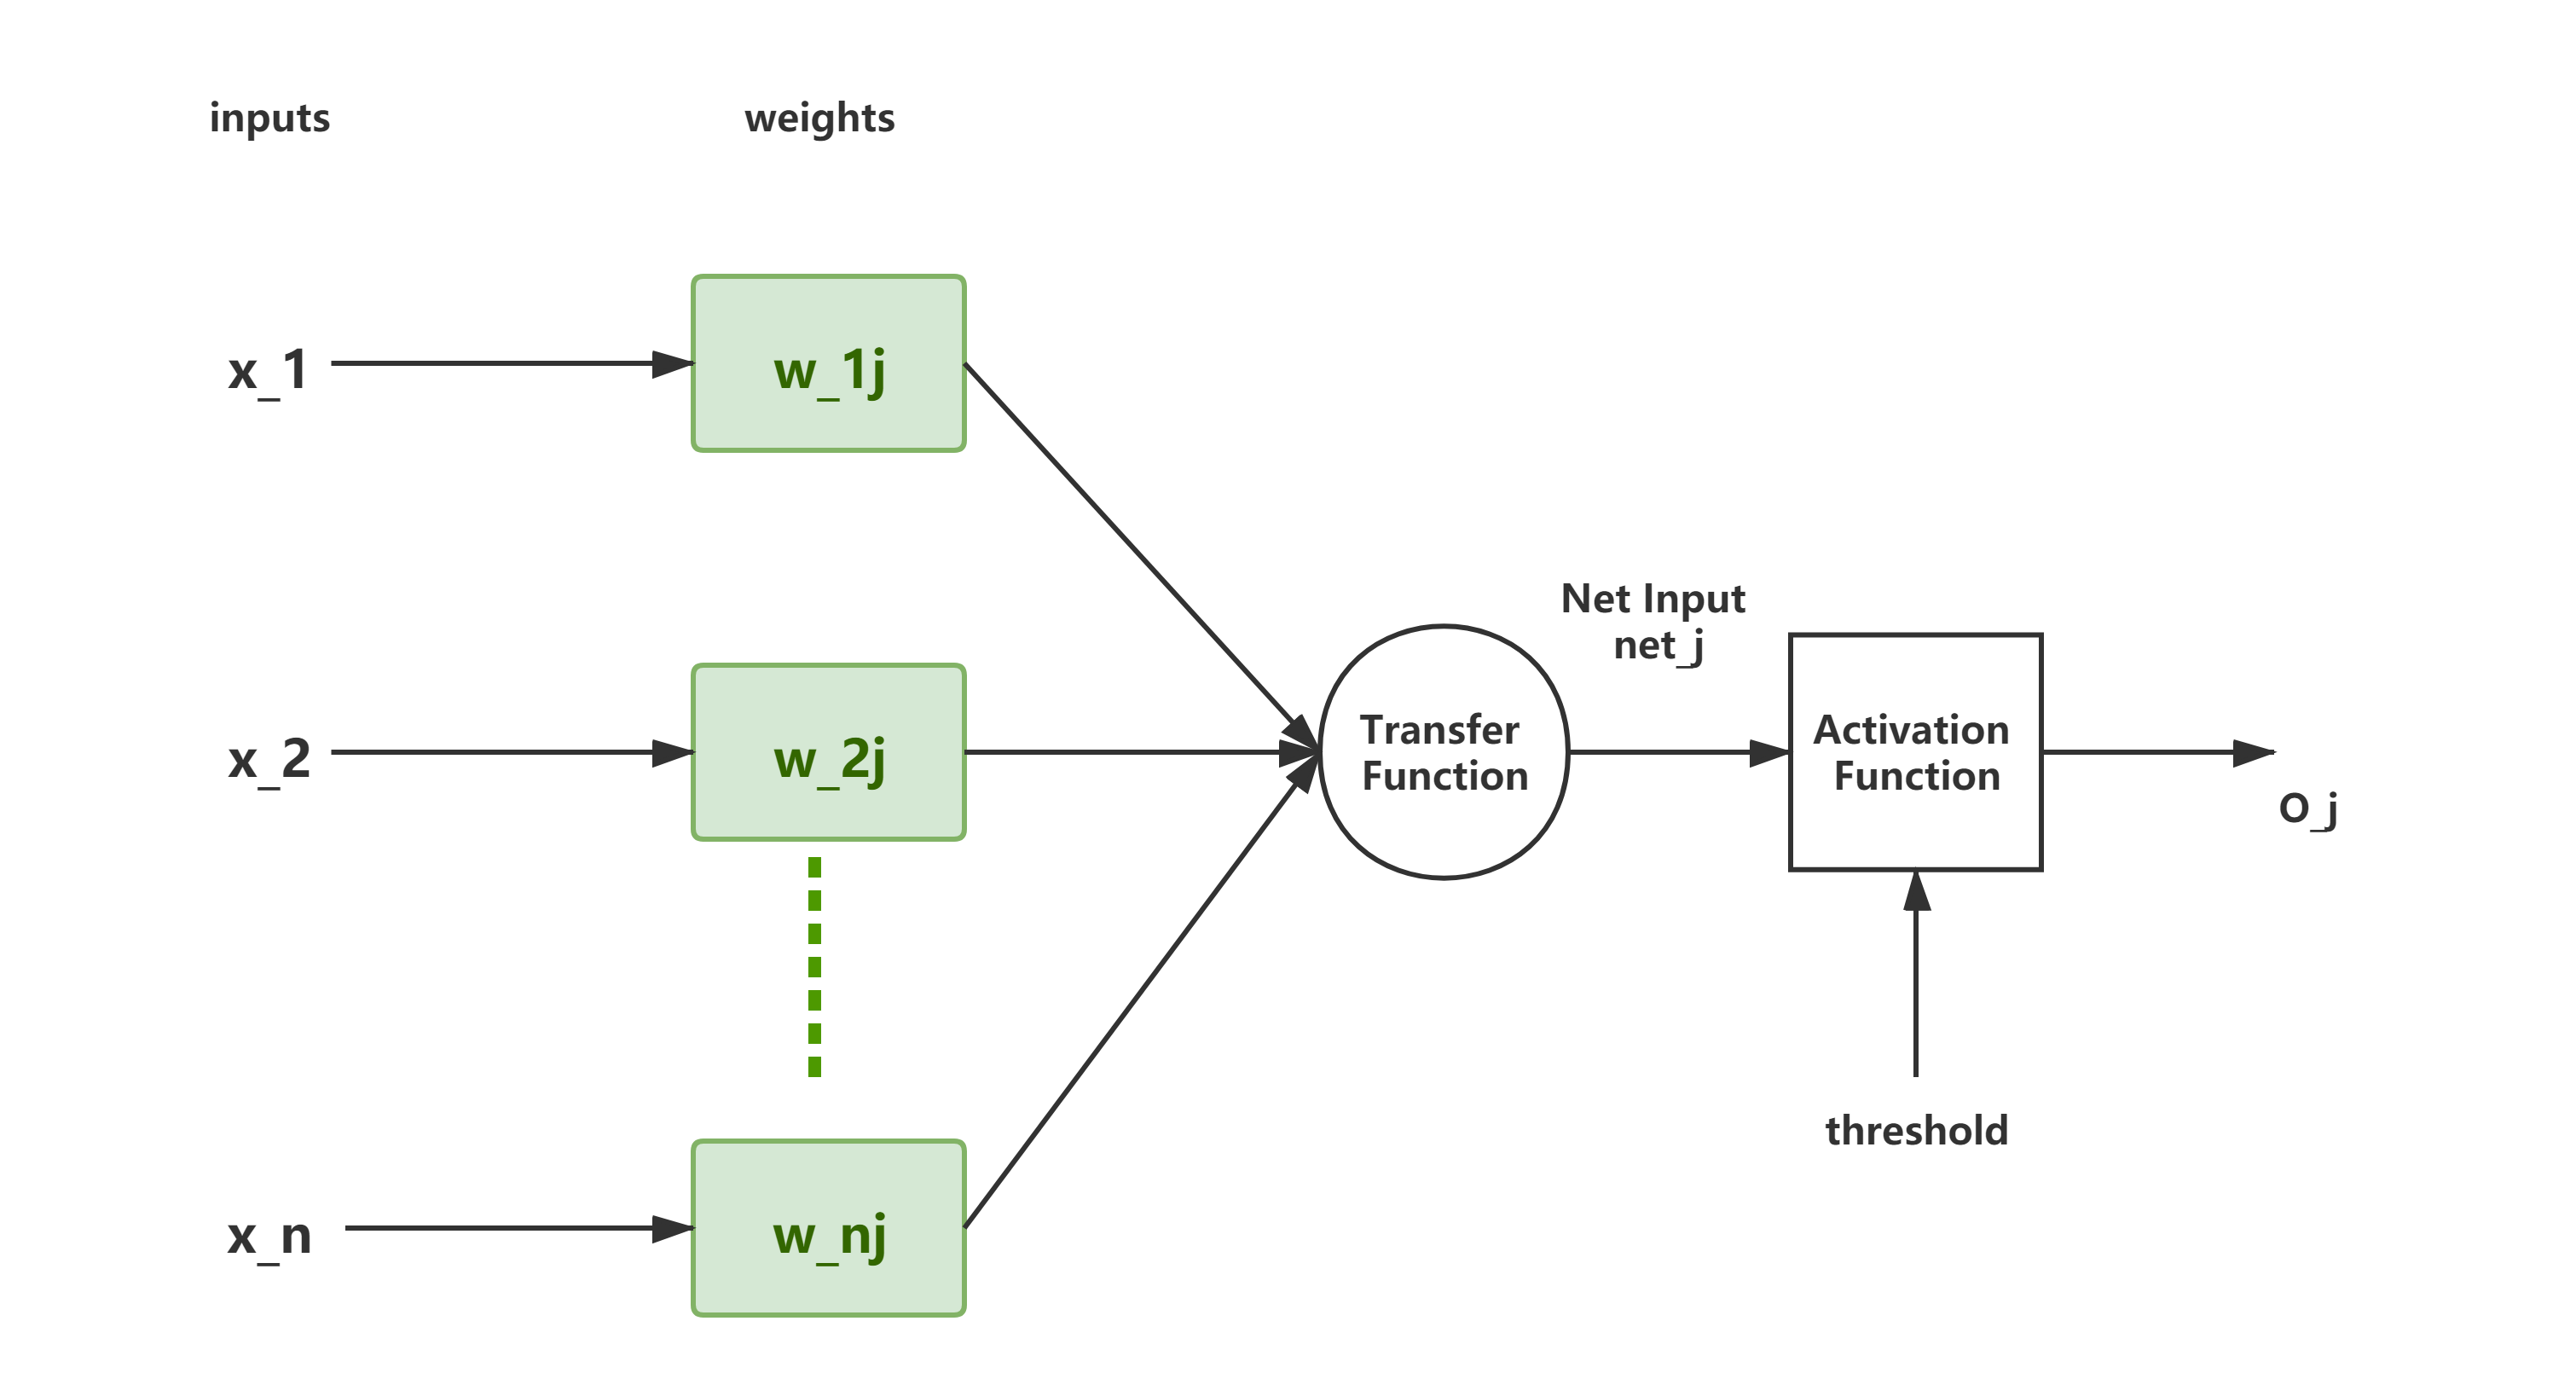
\includegraphics[width=0.9\textwidth]{./images/neuron.png}
\caption{Aritifical Neuron}
\label{fig:neuron}
\end{figure}
Artificial neuron defines the core module of neural network, in addition to weighted input, it also contains transfer and activation functions. Figure \ref{fig:neuron} diagrams an aritificial neuron. The input and output of neuron are $x_1, x_2, \dots, x_N$ and $o_J$, respectively. The output is obtained by calculation and processing of an activation function and a transfer function. The transfer function usually uses the weighted sum function defined below:
\begin{equation}
\text { net }_{j}=\sum_{i=1}^{n} w_{i j} x_{i}
\end{equation}

Then the result of transfer function inputs to activation function. Based on different goal of application, related activation function will be used to calculate the output $o_j$, the general formula is as follows:
\begin{equation}
o_j = f(net_j)
\end{equation}

There are many different activation functions such as sigmoid, softmax, relu and tanh. The corresponding activation function is used in specific application scenarios(e.g. classification or regression).

\subsection{Multi-Layers Neural Network}
In addition to the input and output layers, there are intermediate layers that do not interact with the external environment. Therefore, these intermediate layers are called hidden layers, and their nodes are called hidden nodes. The addition of hidden layers expands the ability of neural networks to solve nonlinear classification problems\parencite{BASHEER20003}. Figure \ref{fig:multi-layer-ann} diagrams a multi-layers neural network.

\begin{figure}[htbp]
\centering
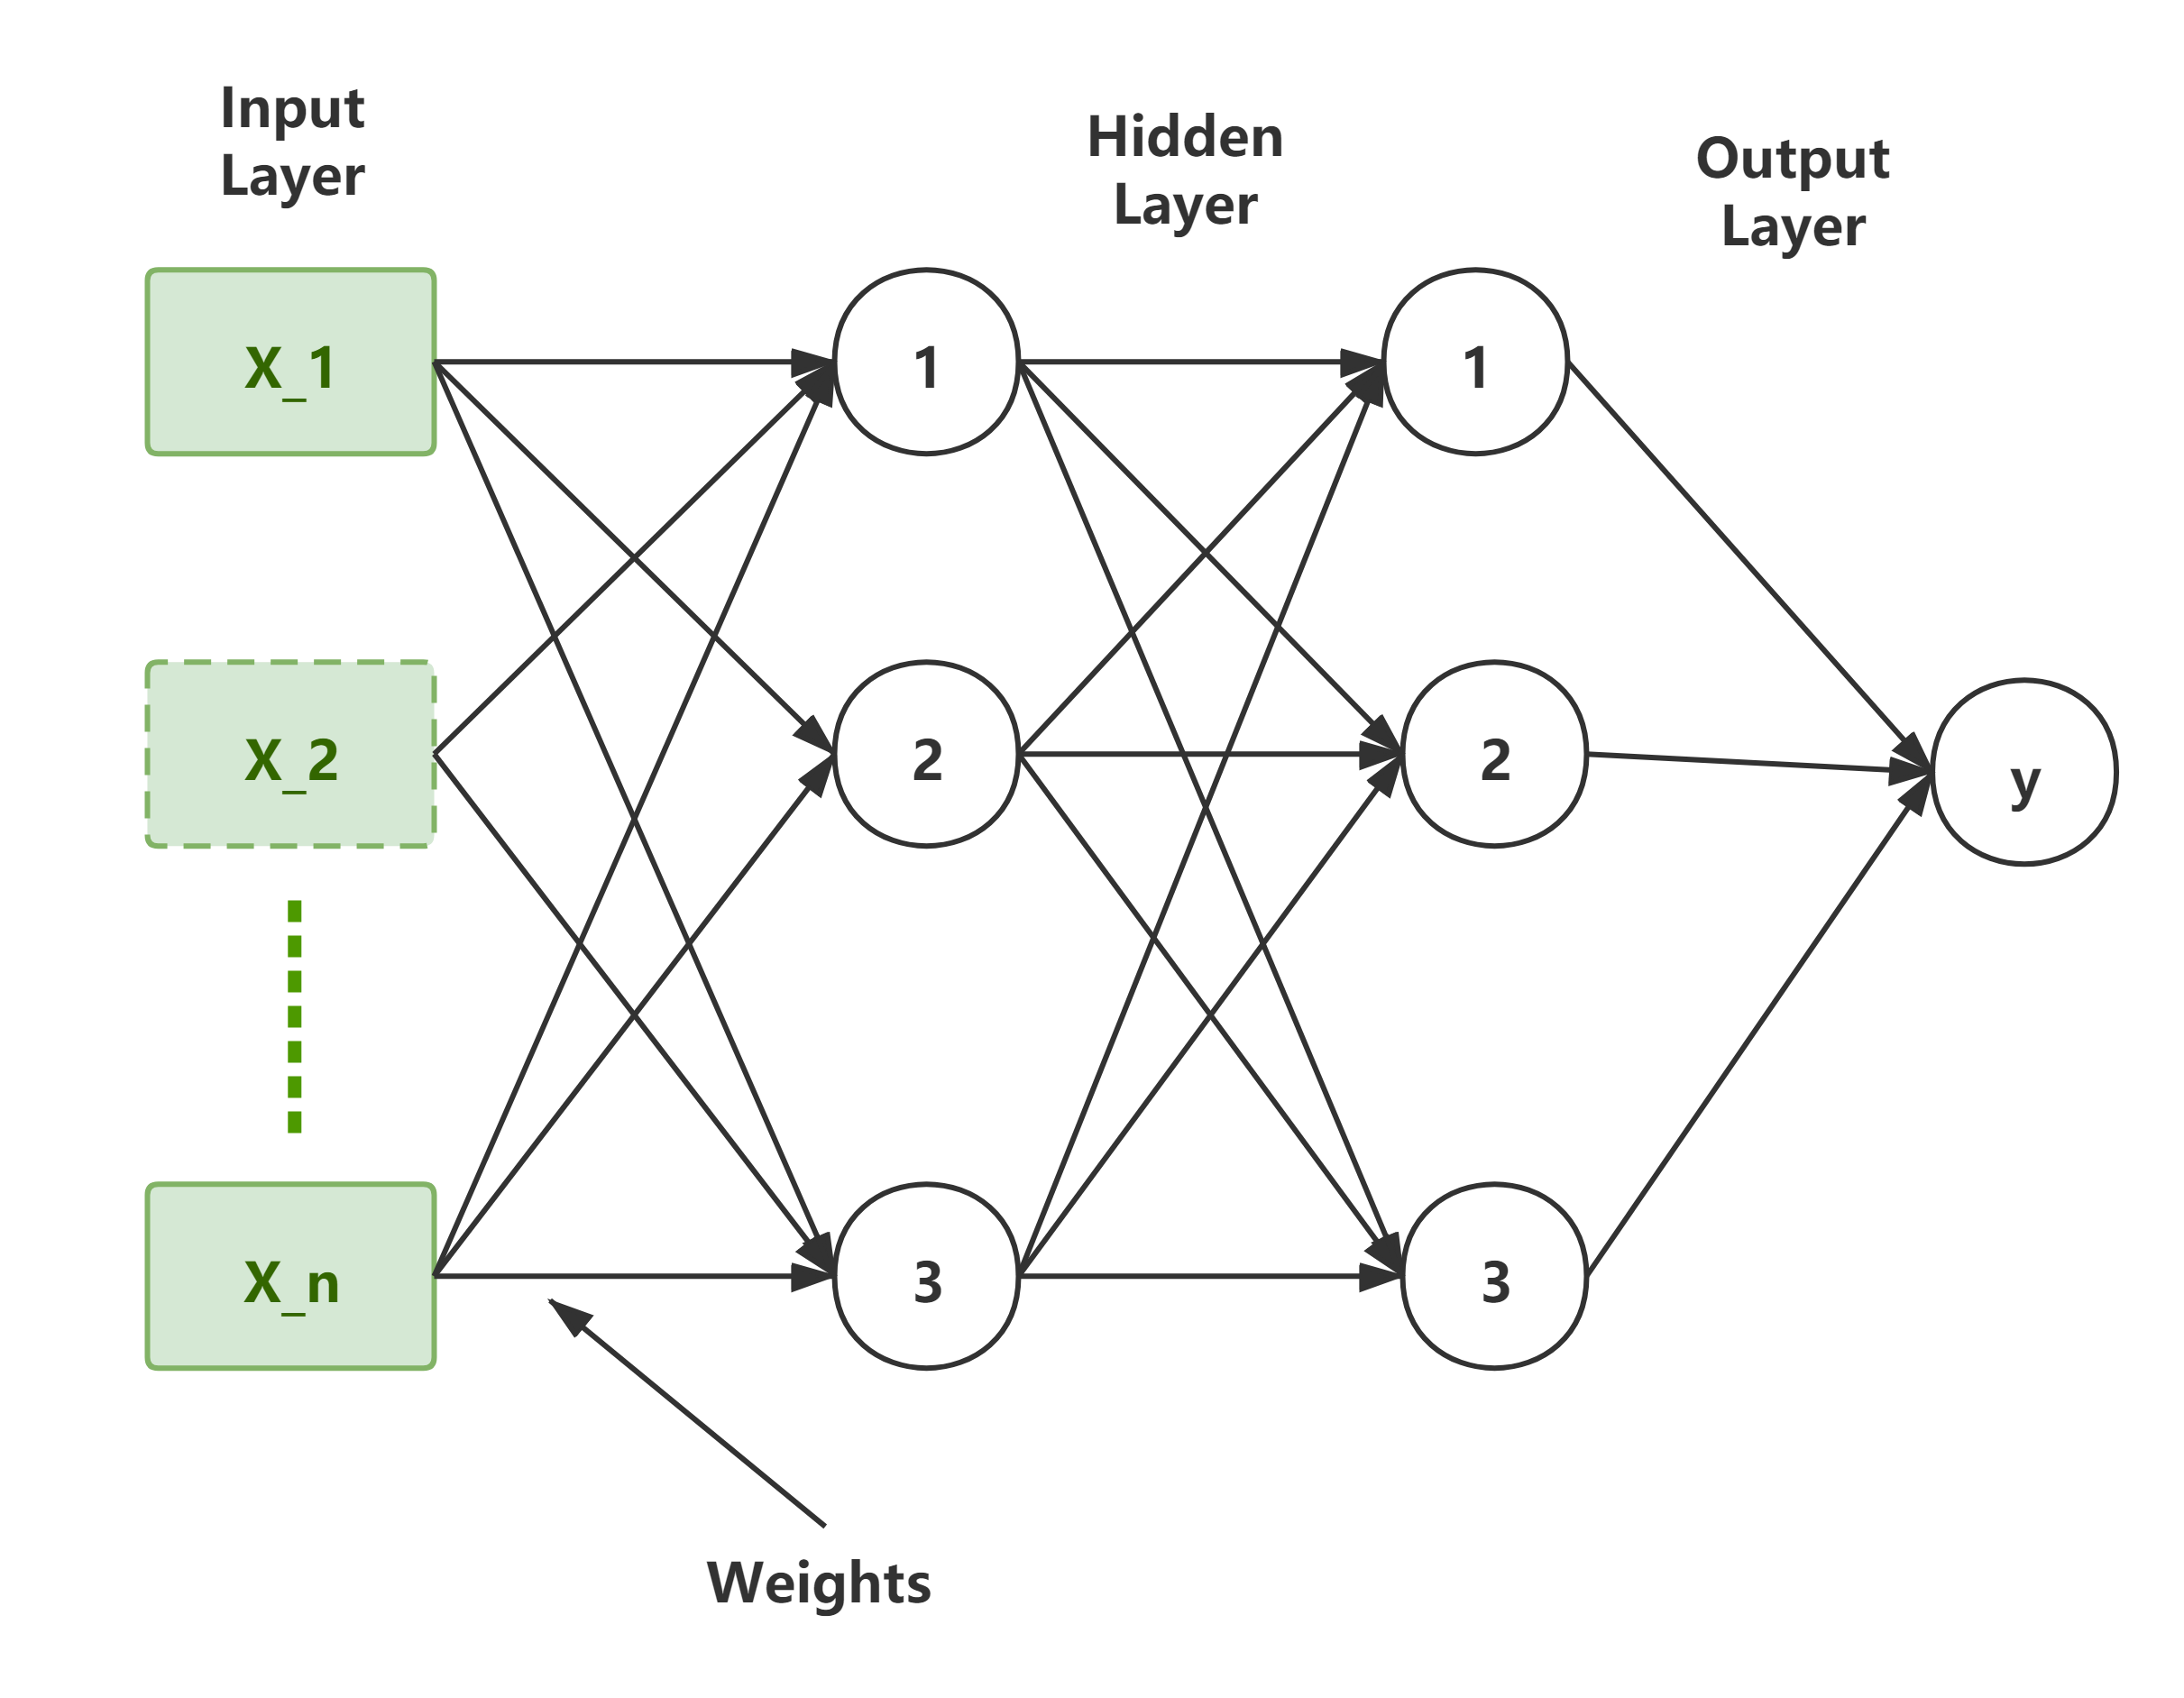
\includegraphics[width=0.9\textwidth]{./images/multi-layer-ann.png}
\caption{Aritifical Multi-Layers Neural Network, x* are inputs. Source: Own illustration based
on\parencite{SAIRAMYA2019253}.}
\label{fig:multi-layer-ann}
\end{figure}

\subsection{Recurrent Neural Networks (RNNS)}
In a recurrent neural network, the output of some neurons are fed back to the same neurons or to neurons in the previous layers\parencite{BASHEER20003}. Information flows both forward and backward directions. These networks have an important ability to store information. The special algorithms for training recurrent networks were introduced in the book \parencite{Hassoun1995}. Figure \ref{fig:recurrent-layer-ann} depicts a recurrent neural networks.

\begin{figure}[htbp]
\centering
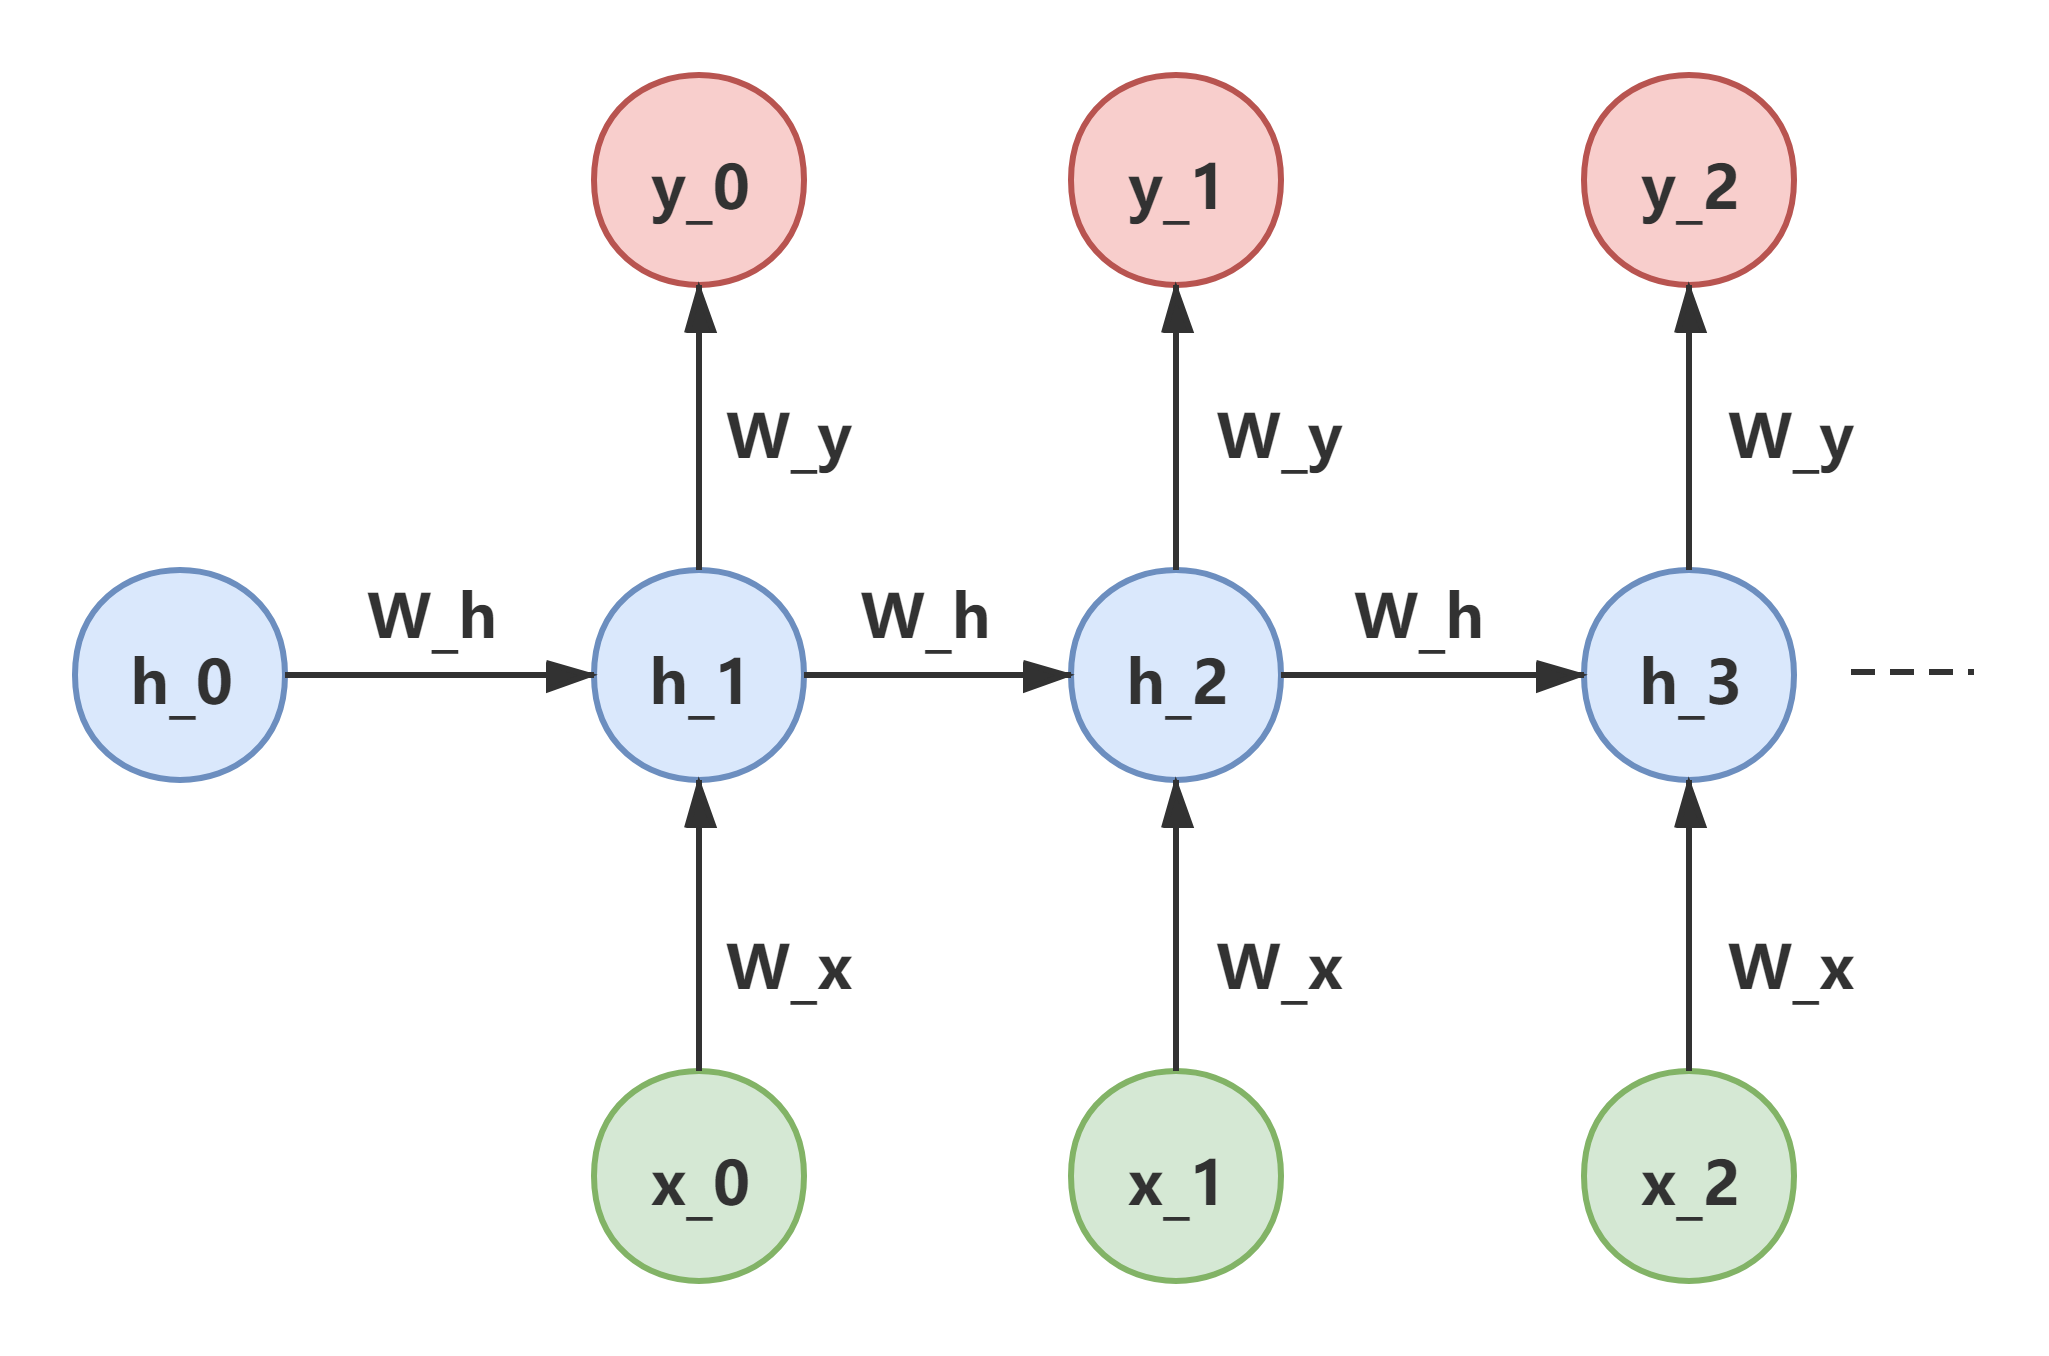
\includegraphics[width=0.9\textwidth]{./images/recurrent-layer-ann.png}
\caption{Recurrent Neural Network where h* are outputs of hidden layers, x* are inputs, y* are outputs of network, w* are the weights corresponding to the layers.}
\label{fig:recurrent-layer-ann}
\end{figure}

\section{Reinforcement Learning}
\subsection{The Agent–Environment Interface}
The reinforcement learning problem is meant to be a straightforward framing of the problem of learning from interaction to achieve a goal. A learner and decision-maker is called an agent. The thing it interacts with, comprising everything outside the agent, is called the environment. These interact continually, the agent selecting actions and the environment responding to those actions and presenting new situations to the agent \parencite{Sutton2018}. Figure \ref{fig:agent-environment-interaction} diagrams the agent–environment interaction.

\begin{figure}[htbp]
\centering
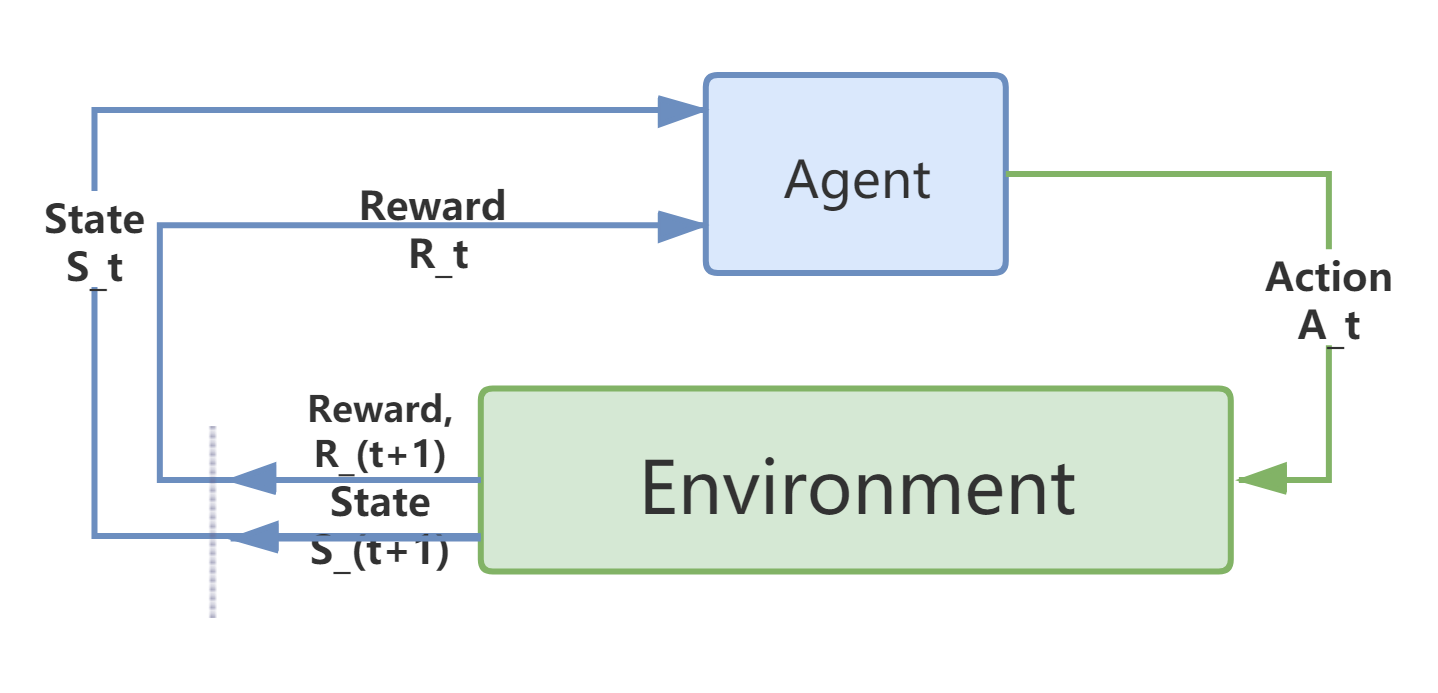
\includegraphics[width=0.5\textwidth]{./images/agent-environment-interaction.png}
\caption{The agent–environment interaction in reinforcement learning, Source: Own illustration based
on\parencite{Sutton2018}.}
\label{fig:agent-environment-interaction}
\end{figure}

Above process is a typical single-agent interaction process. Single-agent reinforcement learning algorithms are based on this process. By extending this interactive process, multi-agent interactive process can be intuitively diagrammed In \ref{fig:multi-agent-environment-interaction}. The case based on multi-agent interaction process is called multi-agent reinforcement learning \gls{marl}. In the figure \ref{fig:multi-agent-environment-interaction}, an agent is splited as two parts: \textbf{perceptor} and \textbf{learner}. \textbf{Perceptor} observes the environment and sends the state to learner. \textbf{Learner} learns strategies based on the states, rewards and actions. There are many methods proposed over the past decade. Some \gls{madrl} methods(e.g., \gls{maddpg}) will be discussed in the following sections. According to the design requirements of the training environment, the structure of the interaction process is flexible.

\begin{figure}[htbp]
\centering
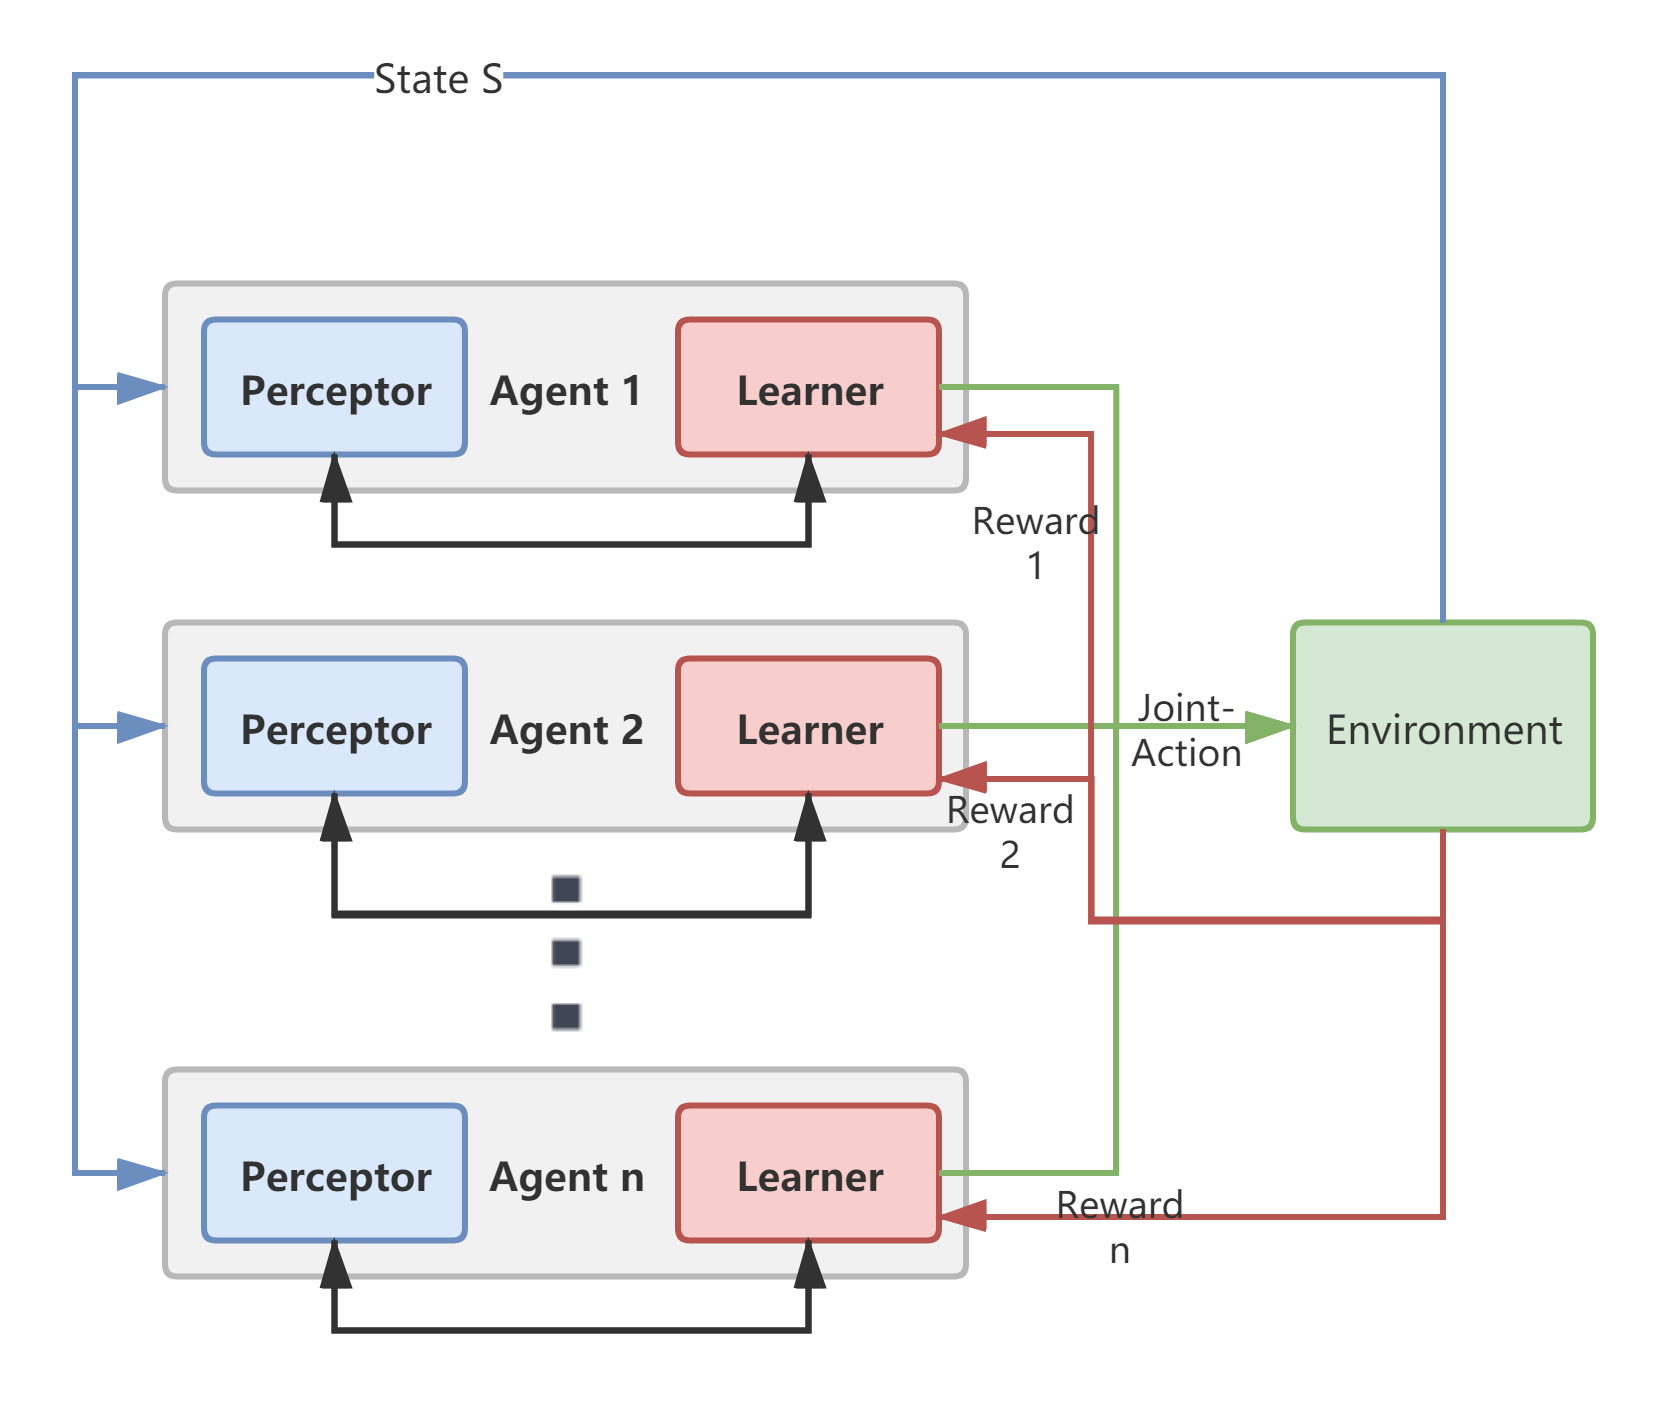
\includegraphics[width=0.6\textwidth]{./images/multi-agent-environment-interaction.png}
\caption{The multi-agent–environment interaction in reinforcement learning, Source: Own illus-
tration based on \parencite{en13010123}.}
\label{fig:multi-agent-environment-interaction}
\end{figure}

\subsection{Value Function} \label{background:value-function}
Just like the description of Markov games in the chapter background \ref{background-game-theory-markov-game}, the agent attempts to find a strategy that maximizes the expected cumulative future discounted reward. The definition of value function stems from this goal of the agent. Value Function can be referred as the state value function and state-action value function which are composed of fixed state or both state and action(state-action pair), respectively.

\textbf{State Value Function($V$)} measures the goodness of each state. It is based on the return reward $G$ following a policy $\pi$. In a formal way, the value of $V_\pi(s)$ is:

\begin{equation} 
V_{\pi}(s)=\mathbb{E}_{\pi}\left[G_{t} \mid S_{t}=s \right]=\mathbb{E}_{\pi}\left[\sum_{j=0}^{T} \gamma^{j} r_{t+j+1} \mid S_{t}=s\right]
\end{equation}
Compared with an infinite \gls{mdp} the time horizon here is set as $T$. The discount is $\gamma$. At the time $t$, $S_t$ denotes the state of agent.

\textbf{State-Action Value Function($Q$)} which measures the goodness of each pair of state and action. Compared with state value function, an action is also determined. The meaning of $G$, $S_t$ and $\gamma$ are same as in the state value function. $A_t$ indicates the action of agent at the time $t$.
\begin{equation}
Q_{\pi}(s, a)=\mathbb{E}_{\pi}\left[G_{t} \mid S_{t}=s, A_{t}=a\right]=\mathbb{E}_{\pi}\left[\sum_{j=0}^{T} \gamma^{j} r_{t+j+1} \mid S_{t}=s, A_{t}=a\right]
\end{equation}

\subsection{Bellman Function}
In summary, bellman function decomposes the value function into two parts: \textbf{immediate reward($r(s, a)$)} and \textbf{discounted future values($\gamma V_{\pi}\left(s^{\prime}\right)$)}.
Equation \ref{equation:bellman-state-value-function} shows how to recursively define the Bellman equation for the state-value function:

\begin{equation} \label{equation:bellman-state-value-function}
V_{\pi}(s)=\sum_{a} \pi(a \mid s) \cdot \sum_{s \prime} P_{s s^{\prime}}^{a}\left(r(s, a)+\gamma V_{\pi}\left(s^{\prime}\right)\right)
\end{equation}
$\pi(a \mid s)$ is the probability that an agent chooses the action $a$ in the state $s$. $P_{s s^{\prime}}^{a}$ is the probability that state of an agent changes from $s$ to $s^{\prime}$ after the agent chooses action $a$.

As same as bellman equation for the state value function, equation \ref{equation:bellman-action-value-function} indicates how to recursively find the q value of a state-action pair following a policy $\pi$.

\begin{equation} \label{equation:bellman-action-value-function}
Q_{\pi}(s, a)=\sum_{s^{\prime}} P_{s s^{\prime}}^{a}\left(r(s, a)+\gamma V_{\pi}\left(s^{\prime}\right)\right)
\end{equation}

\subsection{Q-Learning}
To maximize the total cumulative reward in the long sequence is the goal of RL-agent. The policy, which maximizes the total cumulative reward is called optimal policy formed as $\pi^*$. Optimal \textbf{State-Action-Value-Function} and optimal \textbf{State-Value-Function} are formed as $Q_\pi^*(s, a)$ and $V_\pi^*(s)$, respectively. The update rule of \textbf{State-Action-Value-Function} is shown below:

\begin{equation}
\begin{aligned}
Q_t(s, a) &= Q_{t-1}(s, a) + \alpha TD_t(s, a) \\
					&= Q_{t-1}(s, a)+\alpha\left(R(s, a)+\gamma \max _{a^{\prime}} Q\left(s^{\prime}, a^{\prime}\right)-Q_{t-1}(s, a)\right)
\end{aligned}
\end{equation}
\gls{td} is the abbreviation of \textbf{Temporal Error}. $R(s, a)+\gamma \max _{a^{\prime}} Q\left(s^{\prime}, a^{\prime}\right)$ denotes the \gls{td} target(target q). Current state-action value is formed as $Q_{t-1}(s, a)$. $Q_t(s, a)$ is updated with the learning rate $\alpha$.

\subsection{Policy Gradient \gls{pg}}
Different from Q-Learning, policy gradient learns the strategy directly based on the gradient of reward function. The policy is usually modeled with a parameterized function respect to $\theta$, $\pi_\theta \left(a \mid s\right)$. The gradient of reward function is shown below:
\begin{equation}
\nabla_{\theta} J(\theta)=\mathbb{E}_{s \sim d^{\pi}, a \sim \pi_{\theta}}\left[\nabla_{\theta} \log \boldsymbol{\pi}_{\theta}(a \mid s) Q^{\boldsymbol{\pi}}(s, a)\right]
\end{equation}

The derivation process is written in the appendix \ref{derivation-process-gradient-pg}.

\subsection{Deep Reinforcement Learning (\gls{drl})}
\subsubsection{Deep Q-Networks}
\gls{dqn} uses a Q-Netowrk to replace the Q-Table in normal Q-Learning. Additionally, the training process is supervised by the target network, and the target network is updated by duplicating the parameters of the current network after the fixed frequency training step. The target $q$ is formed as $y_{i}=\left\{\begin{array}{cc}r_{i} & \text { if episode terminates at step } \mathrm{i}+1 \\ r_{j}+\gamma \max _{a^{\prime}} \hat{Q}\left(s_{i+1}, a^{\prime} ; \theta^{-}\right) & \text {otherwise }\end{array}\right.$.

The loss function of \gls{dqn} is shown in the following equation:

\begin{equation}
\mathcal{L}(\theta)=\sum_{i=1}^{T}\left[\left(y_{i}-Q(s, a \mid \theta)\right)^{2}\right]
\end{equation}

$\theta^{-}$ and $\theta$ are the parameters of target network and current network, respectively. The detailed information of the algorithm is described in appendix \ref{appendix:dqn}.

\subsubsection{Proximal Policy Optimization (\gls{ppo})}
During the training process, \gls{pg} will continuously update the probability distribution of actions. However, there is a problem: if the reward is always positive or negative, some possible actions will disappear and it is difficult to sample these actions. \gls{ppo} uses some constraint tricks, such as clip of policy, to avoid this problem. It makes the probability distribution of actions more reasonable. The loss function based on PPO-clip is as follows:
\begin{equation}
L\left(s, a, \theta_{k}, \theta\right)=\min \left(\frac{\pi_{\theta}(a \mid s)}{\pi_{\theta_{k}}(a \mid s)} \hat{A}^{\pi_{\theta_{k}}}(s, a), \quad \operatorname{clip}\left(\frac{\pi_{\theta}(a \mid s)}{\pi_{\theta_{k}}(a \mid s)}, 1-\epsilon, 1+\epsilon\right) \hat{A}^{\pi_{\theta_{k}}}(s, a)\right)
\end{equation} 

The details of algorithm is introduced in appendix \ref{appendix-algorithm-ppo}.

\subsubsection{\gls{dpg},\gls{ddpg}, \gls{maddpg}} \label{background:maddpg}

\textbf{\gls{dpg}}: Deterministic policy gradient creates a $\mu$ function to determine the action instead sampling the action from probability distribution in \gls{pg}.

\textbf{\gls{ddpg}}: DDPG\parencite{Lillicrap2015}, abbreviation for Deep Deterministic Policy Gradient, is a model-free off-policy actor-critic algorithm, combining DPG with DQN. The original DQN works in discrete space, and DDPG extends it to continuous space with the actor-critic framework while learning a deterministic policy. Actor-Critic framework will create two networks named as actor network, which outputs the action, and critic network, which conducts the training and update of actor network.

\textbf{\gls{maddpg}}: Multi-Agent DDPG\parencite{maddpg2017} extends DDPG to an environment where multiple agents coordinate only local information to complete tasks. From the perspective of an agent, the environment is unstable because the policies of other agents will quickly escalate and remain unknown. MADDPG is a critical model of actors, which has been redesigned to deal with this ever-changing environment and the interaction between agents. 

\textbf{Actor update} The gradient of reward of MADDPG is shown below:

\begin{equation}
\nabla_{\theta_{i}} J\left(\boldsymbol{\mu}_{i}\right)=\mathbb{E}_{\mathbf{x}, a \sim \mathcal{D}}\left[\left.\nabla_{\theta_{i}} \boldsymbol{\mu}_{i}\left(a_{i} \mid o_{i}\right) \nabla_{a_{i}} Q_{i}^{\mu}\left(\mathbf{x}, a_{1}, \ldots, a_{N}\right)\right|_{a_{i}=\boldsymbol{\mu}_{i}\left(o_{i}\right)}\right]
\end{equation}
Where $D$ is the memory buffer for experience replay, containing multiple episode samples.

\textbf{Critic update} Loss function is used for updating of critic network. The form of loss function is shown as follow:
\begin{equation}
\mathcal{L}\left(\theta_{i}\right)=\mathbb{E}_{\mathbf{x}, a, r, \mathbf{x}^{\prime}}\left[\left(Q_{i}^{\boldsymbol{\mu}}\left(\mathbf{x}, a_{1}, \ldots, a_{N}\right)-y\right)^{2}\right], \quad y=r_{i}+\left.\gamma Q_{i}^{\boldsymbol{\mu}^{\prime}}\left(\mathbf{x}^{\prime}, a_{1}^{\prime}, \ldots, a_{N}^{\prime}\right)\right|_{a_{j}^{\prime}=\boldsymbol{\mu}_{j}^{\prime}\left(o_{j}\right)}
\end{equation}
Where $\mu^{\prime}$ is the target network(policy) with delayed updated parameters.

The detailed information about the \gls{dpg}, \gls{ddpg} and \gls{maddpg} is introduced in appendix \ref{appendices-algorithms} and \ref{appendices-derivation-process}.

\subsubsection{Value Decomposition Networks(\gls{vdn})}
For multi-agent deep reinforcement learning, there is a very natural idea, which is to learn concentrated state action values but perform action through local observation to solve the non-stational environmemt problem which exists in the scneario, where agents use independet learning methods. The key idea of \gls{maddpg} is the same. However, it has been proven that its convergence is problematic, and training is extremely difficult. This requires on policy learning, which is sample inefficiency, and when there are too many agents, it becomes impractical to train fully focused critics. \gls{vdn}\parencite{Sunehag2017} takes an approach, which learns a centralised but factored $Q_{tot}$. Author represents $Q_{tot}$ as a sum of individual value functions $Q_a$. Each agent selected actions greedily with respect to its $Q_a$. However, a simple summation operator limits the representation ability of centralised action-value function. More importantly, additional environmental states are not considered during the training process.

\subsubsection{\gls{qmix}}
\gls{qmix} is a method first proposed in the paper \texttt{Monotonic Value Function Factorisation for Deep Multi-Agent Reinforcement Learning}\parencite{Rashid2018}. It is used to solve the limitation of \gls{vdn}. \gls{qmix} consists of two networks, one of which is called as agent network representing each $Q_a$, second network is a mixing network that combines all $Q_a$ into $Q_{tot}$, not as a simple sum as in \gls{vdn}. Mixing network uses complex non-linear way to ensure consistency between centralized and decentralized strategies. The detailed model will be introduced in the experiment when it is combined with the experimental environment \ref{methods:qmix-scml-oneshot}.

\section{Platform and Library}
\subsection{GENIUS}
\textbf{GENIUS:} An integrated environment for supporting the design of generic automated negotiators \parencite{Lin2014}.

\subsection{\gls{negmas}} \label{background:negmas}
\gls{negmas} is an opensource automated negotiation platform, which can model situated simultaneous negotiations such as \gls{scm} which will be discussed separately in detail in the next section \ref{background-scml}. The purpose of this section is to provide an overview of the key components(e.g. Mechanism, World) of this platform.

\gls{negmas} is a python library for developing autonomous negotiation agents embedded in simulation environments. The name negmas stands for either \textbf{NEGotiation MultiAgent System} or \textbf{NEGotiations Managed by Agent Simulations}. The main goal of NegMAS is to advance the state of the art in situated simultaneous negotiations. Nevertheless, it can; and is being used; for modeling simpler bilateral and multi-lateral negotiations, preference elicitation , etc \parencite{Mohammad2019}.

\paragraph{\gls{negmas} and Mechanism}
\gls{negmas} has natively implemented five mechanism, Stacked Algernating Offers Mechanism (\gls{saom}), single-text negotiation mechanisms(st) \parencite{raiffa1982art}, multi-text mechanisms(mt)\ref{}, GA-based negotiation mechanisms\parencite{2015effects} and chain negotiations mechasnim(chain of bilateral negotiations). Among them, \gls{saom} is the negotiation mechanism that is discussed and used in the experiments of this thesis. It has been introduced in detail in section Autonomous Negotiation \ref{background:saom}. At the same time, in the related negotiation mechanism packages, some negotiators, such as AspirationNegotiator in negmas.sao, are developed as key part of the packages. These negotiation negotiator will be used as the baseline negotiators in the following experiments.
\paragraph{\gls{negmas} and World}
A simulation is an embedded domain in which agents behave. It is represented in \gls{negmas} by a \textbf{World}. The world in \gls{negmas} was designed to simply the common tasks involved in constructing negotiation driven simulations\parencite{Mohammad2019}. The entire simulation includes multiple simulation steps which is different with the negotiation rounds definied in \ref{background:autonmous-negotiation:basic-notation}. A simulation step can have multiple negotiation rounds. In each step, agents can be allowed to take proactive actions by performing operations worldwide, reading their status from the world, or requesting/operating negotiations with other agents.
\paragraph{\gls{negmas} and Negotiator} Negotiator is an entity in a negotiation mechanism. Several negotiators are natively implemented in \gls{negmas}. AspirationNegotiator, SimpleTitForTatNegotiator and PassThroughSAONegotiator are negotiators, which are developed for \gls{saom}.

The overview of the main components of a simulation in a \gls{negmas} world is shown in Figure \ref{fig:overview-negmas}.

\begin{figure}[htbp]
\centering
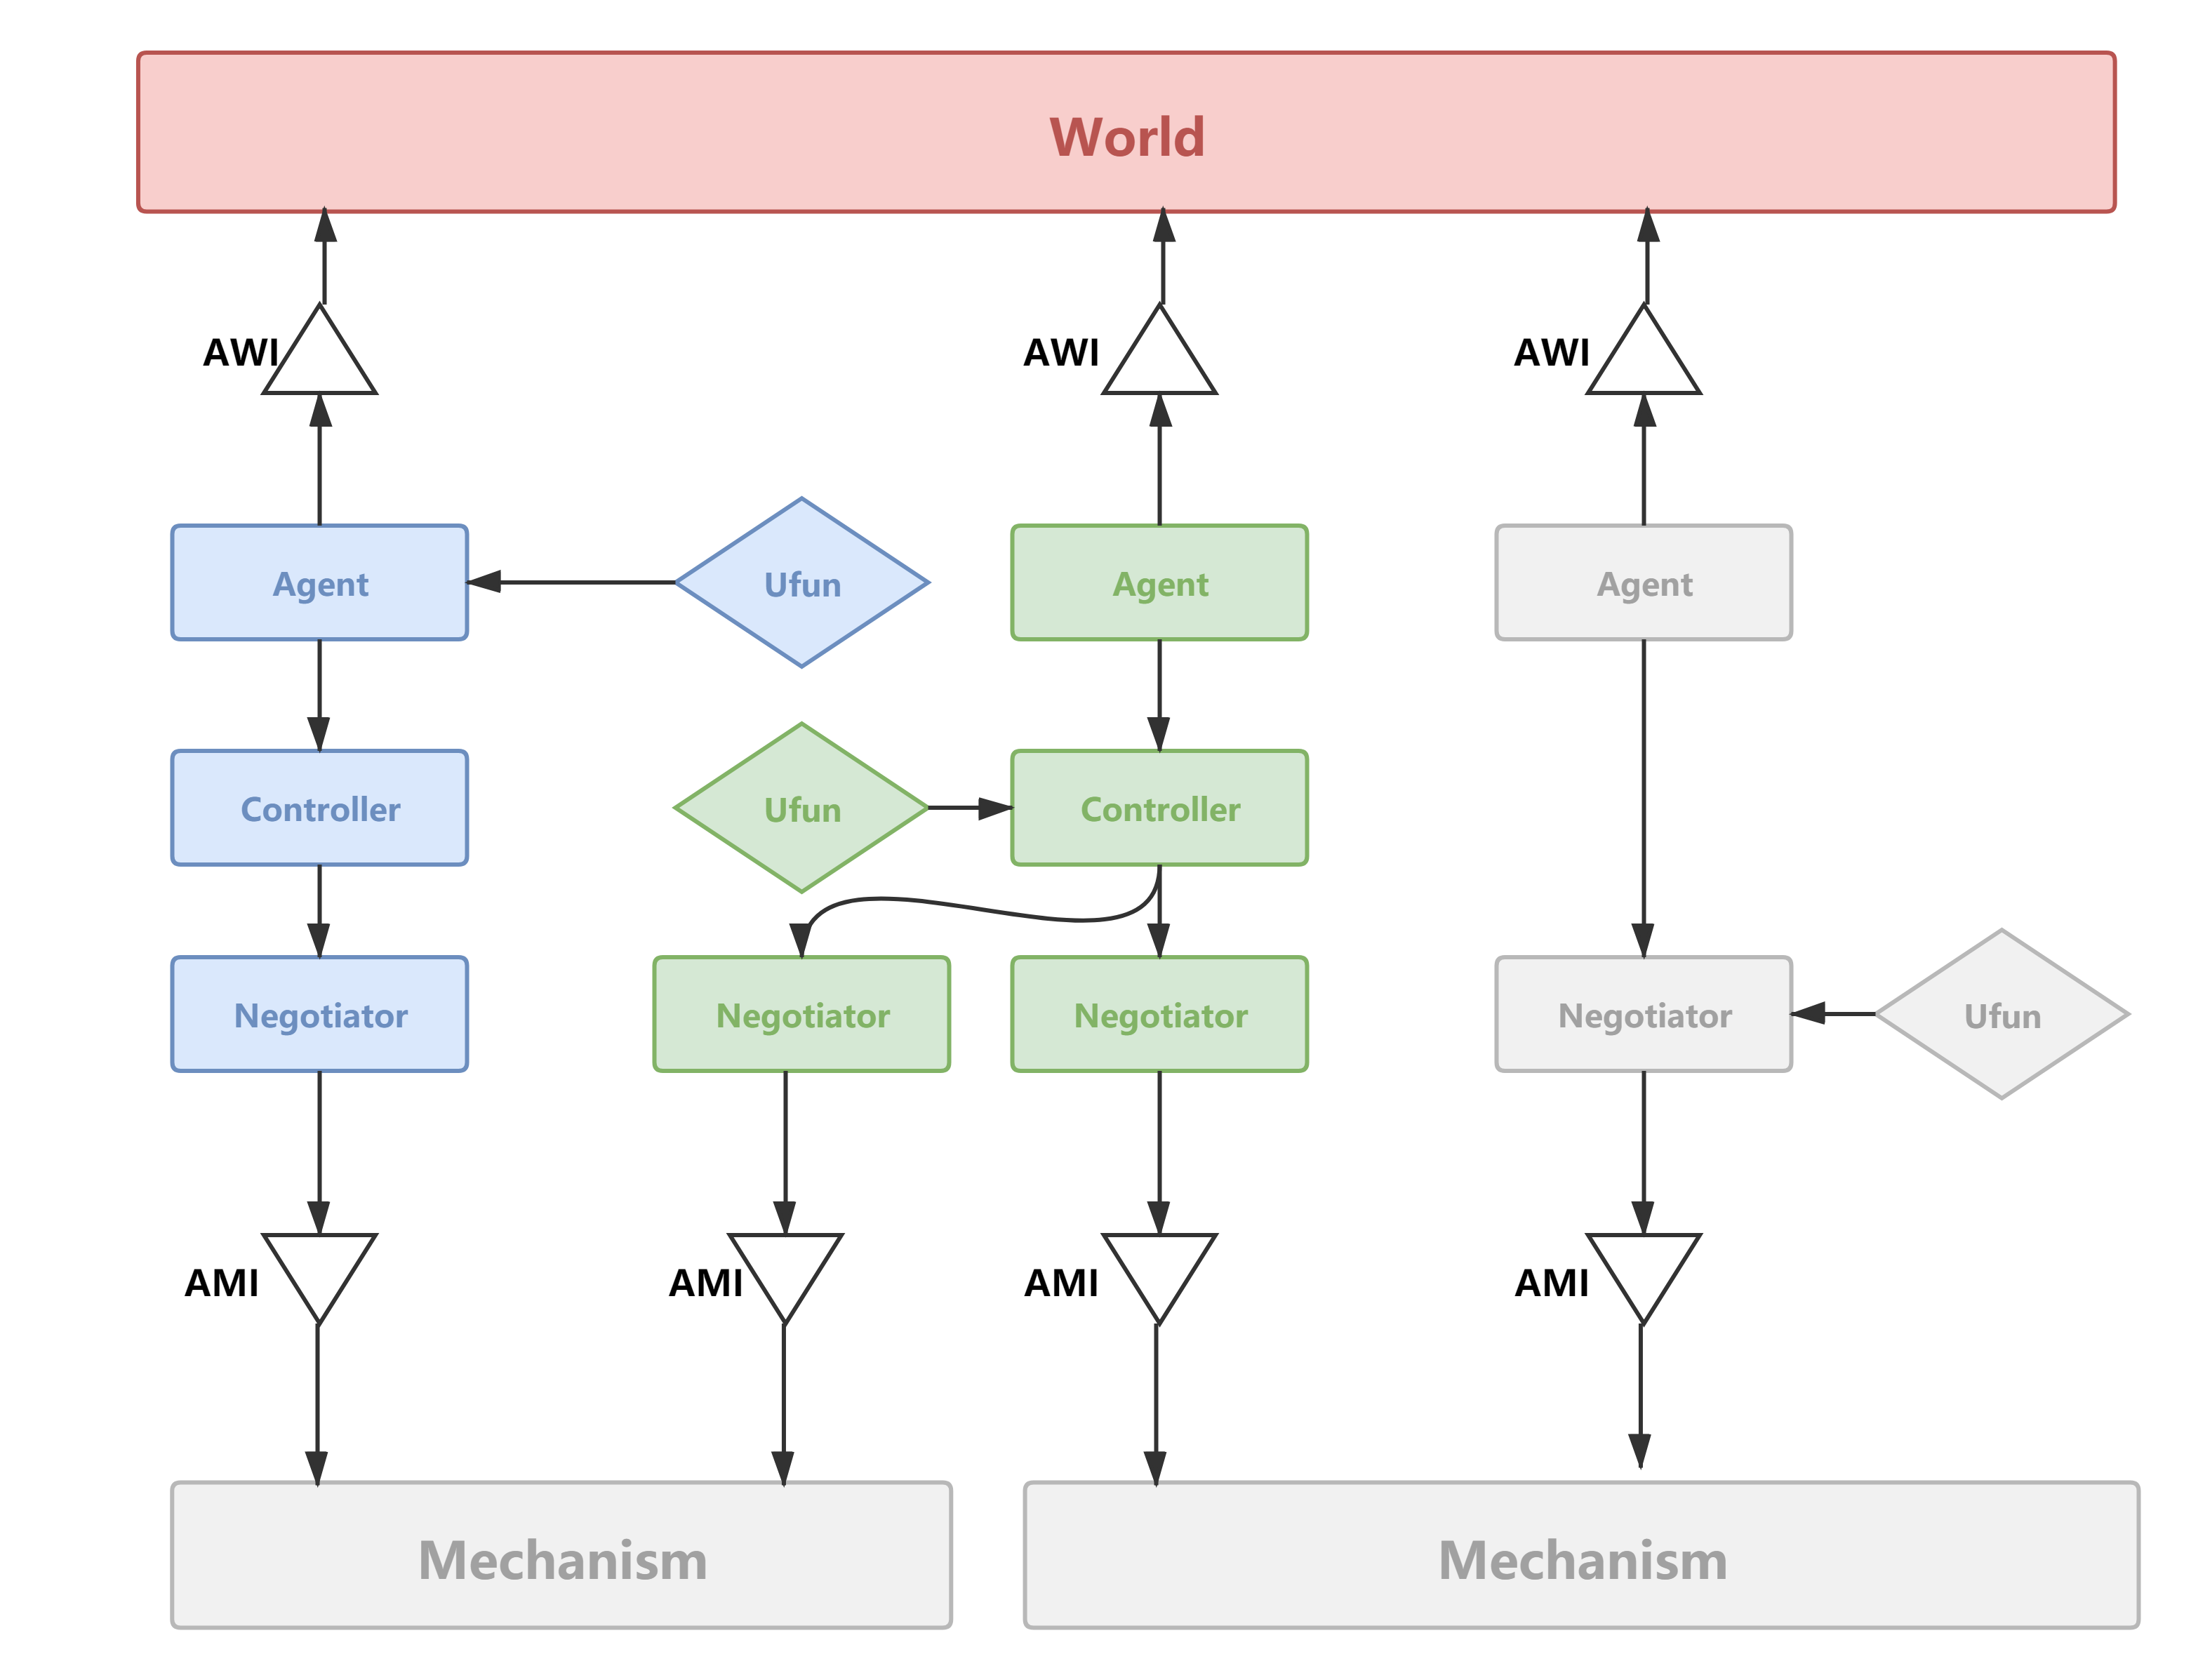
\includegraphics[width=0.8\textwidth]{./images/overview-negmas.png}
\caption{Main components and interactive logic of a simulation in a \gls{negmas} world, \\
Source: Own illustration based on\parencite{Mohammad2019}}
\label{fig:overview-negmas}
\end{figure}

\subsection{\gls{scml}} \label{background-scml}
A supply chain is a sequence of processes by which raw materials are converted into finished goods. A supply chain is usually managed by multiple independent entities, whose coordination is called \textbf{supply chain management(\gls{scm})}. SCM exemplifies situated negotiation. The SCM world was built on top of  \gls{negmas} to serve as a common benchmark environment for the study of situated negotiation \parencite{Mohammad2019}. This repository is the official platform for running \gls{anac} Supply Chain Management Leagues. It will contain a package called scmlXXXX for the competition run in year XXXX. So far, there are three main different versions of \gls{scml} with different designs. In the following sections, some of the components of the three versions related to the work of this thesis will be introduced. 

\begin{itemize}
	\item SCML2020-OneShot: Agent Competition (\gls{anac}) Supply Chain Management League OneShot trace (\gls{scml-oneshot}).
	\item SCML2020/2021: Standard Automated Negotiation Agent Competition (ANAC) Supply Chain Management League (\gls{scml}) 2020/2021.
	\item SCML2019: Standard Automated Negotiation Agent Competition (ANAC) Supply Chain Management League (\gls{scml}) 2019
\end{itemize}

\subsubsection{SCML2020/2021(standard scml)} \label{background:scml2020}
\gls{scml} was originally developed as a part of \gls{negmas}, from the version 0.4.0 it was splited as an indepedent project to research \gls{scm}. \gls{scml} realized a \gls{scm} world to simulate the \gls{scm} process. In this world, agent needs to buy input material through negotiation, manufacture them, then sell output products through negotiation\parencite{Mohammad2021}. The strategy of an agent can be splitted as three parts: \textbf{Trading Strategy}, \textbf{Negotiation Control Strategy}, \textbf{Production Strategy}.

\paragraph{Trading Strategy} determines the quantity(and price) bought and sold at each time step.
\paragraph{Negotiation Control Strategy} this component is responsible for actively requesting negotiation, responding to negotiation requests and actually conducting concurrent negotiation.
\paragraph{Production Strategy} decides what to produce at every time-step.

\subsubsection{SCML2020-OneShot} \label{background:scml2020-oneshot}
In \gls{scml-oneshot} world, the simulation steps can be referred as days. There are multiple concurrent negotiations going on every day. Difference with the SCML2019 and SCML2020/2021, \gls{scml-oneshot} emphasizes negotiation and de-emphasizes operations (e.g. scheduling) which are also important in standard scml. The simulation in oneshot focuses on the research of concurrent negotiation. The design of \gls{scml-oneshot} ensures the following points \parencite{Mohammad2021}:

\begin{itemize}
	\item Agents (factory managers) consider only the negotiations in the current simulation step. Only the current concurrent negotiations can affect the agent's score. It means, regardless of the result of the negotiations, the concurrent negotiations will be ended at the end of the simulation step. 
	\item Agents can learn over time about their negotiation partners (i.e. suppliers or consumers).
\end{itemize} 

Figure \ref{fig:overview-scml-oneshot} diagrams a World created by \gls{scml-oneshot}

\begin{figure}[htbp]
\centering
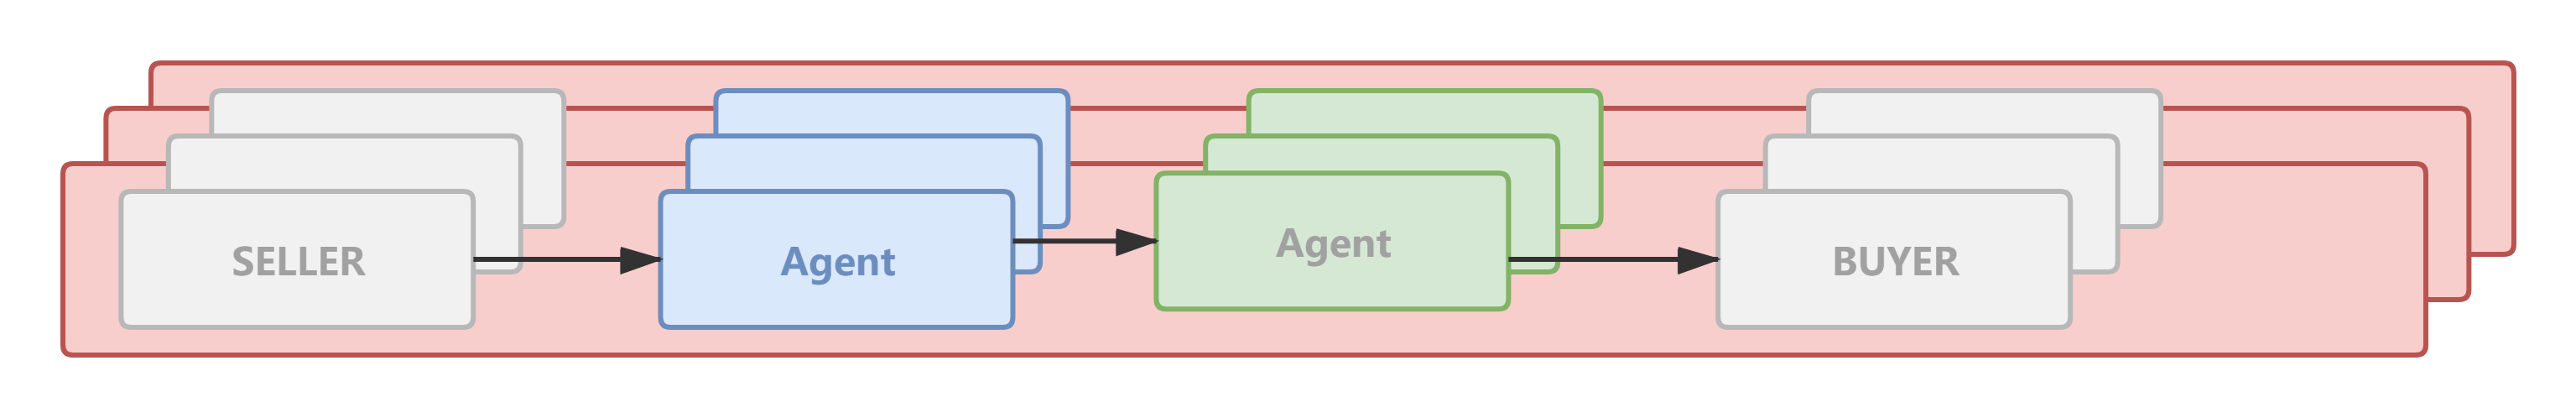
\includegraphics[width=0.8\textwidth]{./images/overview-scml-oneshot.png}
\caption{Main running logic of a simulation in a \gls{scml-oneshot} world, Each red box represents a day. Broken lines represent exogenous contracts while connected lines are negotiations (about the intermediate product). All negotiations conducted in a given day are about deliveries on the same day. Source: Own illustration based on\parencite{Mohammad2021}}
\label{fig:overview-scml-oneshot}
\end{figure}

\paragraph{Production Graph} defines the products defined in the world and the process of converting between them. There are three product types: raw-material, intermediate-product and final-product and two manufacting processes for converting the raw materail into the intermediate product and for converting the intermediate product to the final product.
\paragraph{Factories} is an entity which in the \gls{scm} world convert input products into output products by running manufacturing process on their production lines. A special point is that all processes require zero time to complete.
\paragraph{Agents} The agents in the \gls{scm} world function as factory managers controlling the negotiations between factories.
\paragraph{Conctracts} include normal contracts which are signed agreements between agents or exogenous contracts, which are contracts signed between agent and system entities(BUYER and SELLER).
\paragraph{Utiliy Function} The utility function of an agent specifies its preferences over possible outcomes of a negotiation. Utility function is well defined in \gls{scml-oneshot}. It is simply the total money it receives minus the money it pays for buying input product, production cost, storage and garbage collection costs and delivery penalties. It is called OneShotUfun in \gls{scml-oneshot} world. This utility can be set as a part of reward function of RL-agent. The complete information of the utility function will be covered in Chapter 4 "Analysis" \ref{analysis:scml:design-of-reward-function}.
\paragraph{Negotiation Mechanism} The negotiation mechanism is a variant of Rubinstein's alternating offers protocol. It involves two agents, who take turns making offers for a finite number of rounds. One agent opens the negotiation with an offer, after which the other agent takes one of the actions(Accepts, Counter-offer, Walks away). All actions are also introduced in SAOM \ref{background:saom}. This process repeats until an agreement or a deadline is reached. A key difference between the variant of the protocol used in the SCM world and other implementations of the alternating offers protocol is that in the first round of negotiations, both agents propose an offer, and then one of these offers is chosen at random to be the initial offer.
\paragraph{Bulletin Board} The world contains a world-readable bulletin board. It contains both static and dynamic information about the game and all factories. The static information includes the game settings, product information, catalog prices and trading prices. The dynamical information includes a breach list and a financial reports.
\paragraph{Simulation World} Each simulation in \gls{scm} world runs for multiple days. Before the first day, each agent is assigned a private production cost $(m_f)$. During each day\parencite{Mohammad2021}:
\begin{itemize}
\item Conduct multiple rounds of negotiations between agents.
\item Execute all contracts.
\item Update the bulletin board to reflect new financial reports, transaction prices and external contract summaries.
\end{itemize}

\subsection{Tensorflow} Tensorflow is an end-to-end open source platform for machine learning. It has a comprehensive and flexible ecosystem of tools, libraries and community resources, allowing researchers to promote the latest developments in ML, and allowing developers to easily build and deploy ML-supported applications\parencite{tensorflow2015-whitepaper}.

\subsection{\gls{pytorch}} PyTorch is an open source machine learning library and framework which performs immediate execution of dynamic tensor computations with automatic differentiation and GPU acceleration, and does so while maintaining performance comparable to the fastest current libraries for deep learning\parencite{NEURIPS2019_bdbca288}. While considering performance, it is also easier to apply and debug.

\subsection{\gls{openai gym}}
\gls{openai gym} is a toolkit for developing and comparing reinforcement learning algorithms \parencite{brockman2016openai}.
\subsubsection{Environment}
The core gym interface is \texttt{Env}, which is the unified environment interface. The following are the Env methods that developers should implement \parencite{brockman2016openai}.

\paragraph{STEP} Run one timestep of the environment's dynamics. When end of episode is reached, \texttt{reset()} is calld to reset this environment's state. Accepts an action and returns a tuple (observation, reward, done, info).
\begin{itemize}
\item observation (object): agent's observation of the current environment, such as frame of the game.
\item reward (float): amount of reward returned after previous action, such as 1 when action is go to left.
\item done (bool): whether the episode has ended, in which case further step() calls will return undefined results, such as agent is dead in game, as True.
\item info (dict): contains auxiliary diagnostic information (helpful for debugging, and sometimes learning), such as goal of agent.
\end{itemize}

\paragraph{RESET} Resets the environment to an initial state and returns an initial observation. This function should not reset the environment's random number generator(s). Random variables in the environment's state should be sampled independently between multiple calls to \texttt{reset()}. Each call of \texttt{reset()} should yield an environment suitable for a new episode, independent of previous episodes.
\paragraph{RENDER} Define how to display the output of the environment. Multiple modes can be used: 
\begin{itemize}
	\item human: Render to the current display or terminal and return nothing. Usually for human consumption
	\item rgb\_array: Return an numpy.ndarray with shape (x, y, 3), representing RGB values for an x-by-y pixel image, suitable for turning into a video.
	\item ansi: Return a string (str) or StringIO.StringIO containing a terminal-style text representation. The text can include newlines and ANSI escape sequences (e.g. for colors).
\end{itemize}

\paragraph{CLOSE} Override close in the subclass to perform any necessary cleanup. Environments will automatically \texttt{close()} themselves when garbage collected or when the program exits. Save datas at the end of the program.
\paragraph{SEED} Sets the seed for this env's random number generator(s). It is useful for reproducing the results.
\begin{lstlisting}[caption={Logic of \gls{openai gym} Interaction},label={lst:openaigym},language=python]
ob0=env.reset() #sample environment state, return first observation
a0=agent.act(ob0) #agent chooses first action
ob1,rew0,done0,info0=env.step(a0) #environment returns observation,
#reward, and boolean flag indicating if the episode is complete.
a1=agent.act(ob1)
ob2,rew1,done1,info1=env.step(a1)
...
a99=agent.act(o99)
ob100,rew99,done99,info2=env.step(a99)
# done99 == True => terminal
\end{lstlisting}

From Listing \ref{lst:openaigym}, user can get the logic of interaction in \gls{openai gym}.

\subsubsection{Stable Baselines} \label{backgrounds:stable-baselines}
The \textbf{Stable Baselines} are developed in the project stable-baselines\parencite{stable-baselines}. The project implemented a set of improved implementations of \gls{rl} algorithms based on OpenAI Baselines\parencite{baselines}. All implemented algorithms with characteristic discrete/continuous actions are shown in \ref{tab:stable-baselines}.

\begin{table}[htbp]
\centering
\begin{tabular}{l l l} \toprule
\bfseries Name       & \bfseries Box  & \bfseries Discrete \\ \midrule
\verb#A2C#                         & Yes  &  Yes \\
\verb#ACER#                  			 & No   &  Yes \\
\verb#ACKTR#                       & Yes  &  Yes \\
\verb#DDPG#                        & Yes  &  No  \\
\verb#DQN#                         & No   &  Yes \\
\verb#HER#                         & Yes  &  Yes \\
\verb#GAIL#                        & Yes  &  Yes \\
\verb#PPO1#                        & Yes  &  Yes \\
\verb#PPO2#                        & Yes  &  Yes \\
\verb#SAC#                         & Yes  &  No  \\
\verb#TD3#                         & Yes  &  No  \\
\verb#TRPO#                        & Yes  &  Yes \\
\bottomrule
\end{tabular}
\caption{stable baselines algorithms}
\label{tab:stable-baselines}
\end{table}

\subsection{\gls{ray}}
An open source framework that provides a simple, universal API for building distributed applications. Ray is packaged with the following libraries for accelerating machine learning workloads\parencite{DBLP:journals/corr/abs-1712-05889}.
\begin{itemize}
	\item Tune: Scalable Hyperparameter Tuning
	\item RLlib: Scalable Reinforcement Learning
	\item RaySGD: Distributed Training Wrappers
	\item Ray Serve: Scalable and Programmable Serving
\end{itemize}



